Originally posted at
\url{http://vinipsmaker.wordpress.com/2013/07/21/splines-extraction-on-kopf-lischinski-algorithm-part-1/}
on \formatdate{21}{7}{2013}.

\subsection{Polygon union}

Polygons can be represented by vertice points. libdepixelize stores them in
clockwise order, with the first point being part of the polygon's
northwest/top-left. One important feature of the generated Voronoi diagram
is that all ``connected'' cells share a common edge.

The algorithm can be described in 4 major steps:

\begin{enumerate}
\item Find the largest common edge
\item Remove the in-between points of the common edge
\item Choose one polygon and refer to it as P (choose the smallest polygon for
  better performance)
  \begin{enumerate}
  \item 
    Shift P such as P's head and tail are points of the common edge
  \end{enumerate}
\item Choose the other and refer to it as Q
  \begin{enumerate}
  \item Remove one of the common edge's points in Q
  \item Replace the remaining point that is part of the common edge in Q by P's
    points
  \end{enumerate}
\end{enumerate}

The Voronoi cells are iterated one by one, line by line, from the left-most cell
to the right-most cell. This behaviour could change in favor of a
\href{http://en.wikipedia.org/wiki/Cache-oblivious_algorithm}{cache-oblivious
algorithm}.

We check if (1) we already have a group of the current color, (2) the existing
group has a common edge with current Voronoi cell and, then, (3) we add the
current Voronoi cell to the existing polygon. Beware that the Voronoi cells from
the input are always convex polygons, but the existing polygon (that groups the
Voronoi cells) might be
\href{http://en.wikipedia.org/wiki/Concave_polygon}{concave}.

Let's see an example of the algorithm. In the example, we are iterating in the
second line and we found an existing grouping polygon with a matching color (the
two entities are connected), then we must add them togheter. The image below
represents the situation we are interested in:

\begin{figure}[H]
  \centering
  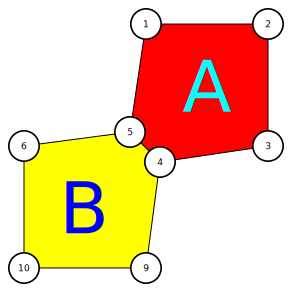
\includegraphics[width=0.8\textwidth]{assets/polygon-union.pdf}
\end{figure}

Polygon A is represented by the list of points [1, 2, 3, \textbf{4}, \textbf{5}]
(common edge's points in bold). Polygon B is represented by the list of points
[6, \textbf{7}, \textbf{8}, 9, 10] (common edge's points in bold). Points 4 and
8 are equal and points 5 and 7 are equal. Polygon A is the grouping polygon
while polygon B is the current Voronoi cell. We shift B's list to [\textbf{8},
9, 10, 6, \textbf{7}] and use it to get the final polygon [1, 2, 3, 8, 9, 10, 6,
7].

Let's do it one more time:

\begin{figure}[H]
  \centering
  \includegraphics[width=0.8\textwidth]{assets/polygon-union2.pdf}
\end{figure}

Polygon A is the grouping polygon, represented by [1, 2, \textbf{3}, \textbf{8},
\textbf{9}, 10, 6, 7]. Polygon C is the current Voronoi cell and is represented
by [\textbf{11}, \textbf{12}, 13, \textbf{14}]. This time the largest common
edge have 3 points and point 8/11 is the in-between point, then we remove it.
The resulting A polygon is [1, 2, \textbf{3}, \textbf{9}, 10, 6, 7] and the
resulting C polygon is [\textbf{12}, 13, \textbf{14}]. When we replace the
common edge interval in A by C, we get the final polygon, [1, 2, \textbf{12},
13, \textbf{14}, 10, 6, 7]. The final polygon is show in the image below:

\begin{figure}[H]
  \centering
  \includegraphics[width=0.8\textwidth]{assets/polygon-union3.pdf}
\end{figure}

One last note that might be useful in later steps is the access pattern used by
the algorithm. When we add a voronoi cell to the grouping polygon, there is a
hot area and a cold area. The cold area is the area where there will never be a
common edge. These areas always are concetrated in the same places, like
exemplified by the following image:

\begin{figure}[H]
  \centering
  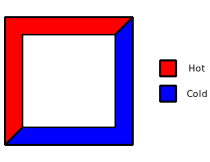
\includegraphics[width=0.8\textwidth]{assets/hot-cold.pdf}
\end{figure}

\subsection{Splines generation}

The previous step look simple, but there may be additional info that we may want to
store for each node. This (polygon-union) is the last step where we still can
gather locality info without executing a deep lookup.

\begin{figure}[H]
  \centering
  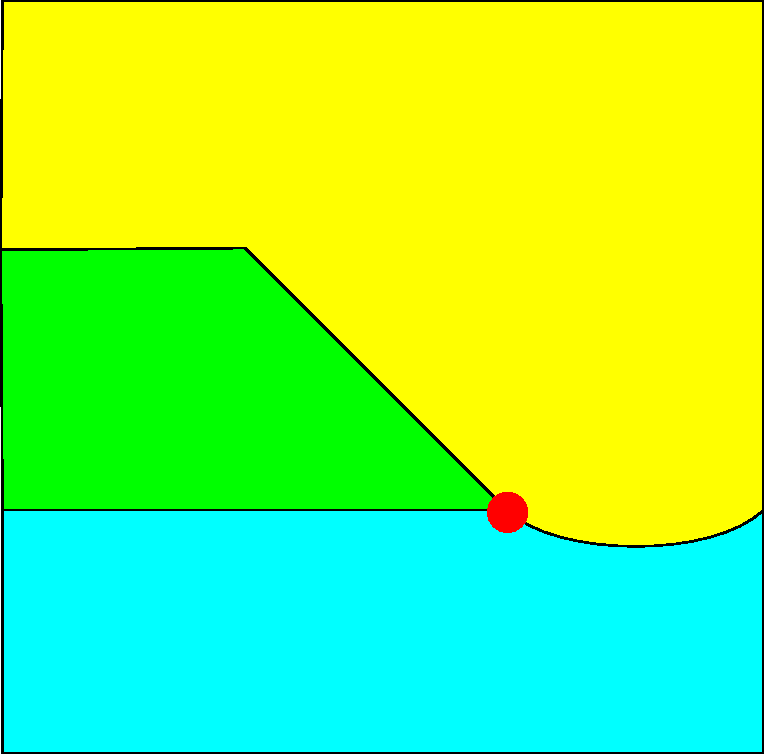
\includegraphics[width=0.8\textwidth]{assets/valence-3-node.pdf}
  \caption{Valence-3 node (in red)}
\end{figure}

Let's refer to nodes where at most two different grouping polygons share a point
as valence-2 nodes. There are valence-2 nodes, valence-3 nodes and valence-4
nodes. Valence-2 nodes are always smooth and valence-4 nodes never are smooth,
but valence-3 nodes vary.

\begin{figure}[H]
  \centering
  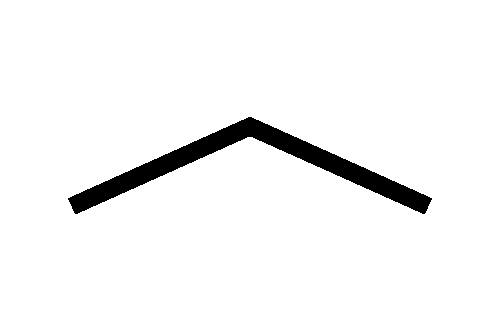
\includegraphics[width=0.8\textwidth]{assets/non-smooth.pdf}
  \caption{Non-smooth node}
\end{figure}

Most of the points are shared by nodes of different polygons and when we have
three valence-3 nodes, exactly only one of them will be smooth. We apply
Kopf-Lischinski algorithm heuristics to determine which one will be and store
this info for later usage.

\begin{figure}[H]
  \centering
  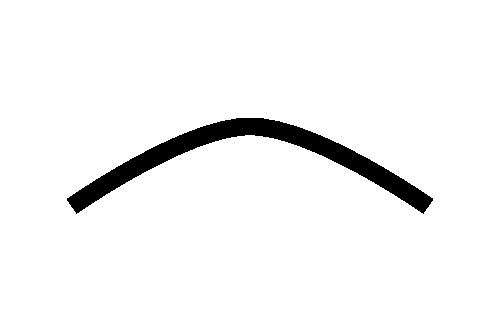
\includegraphics[width=0.8\textwidth]{assets/smooth.pdf}
  \caption{Smooth node}
\end{figure}

The complicated part about the splines extraction on Kopf-Lischinski algorithm
is the overlapping between these last steps (group the Voronoi cells to identify
visible edges and generate the splines).

\subsection{A bit of performance}

So, Kopf-Lischinski algorithm resembles a compiler. You have several data
representation types and each type offers different operations. You explore the
operations each type offers and convert it to another representation until you
reach the final result. In several of the type representations used by the
Kopf-Lischinski algorithm, you have a matrix and you access each element and its
neighbours.

\begin{figure}[H]
  \centering
  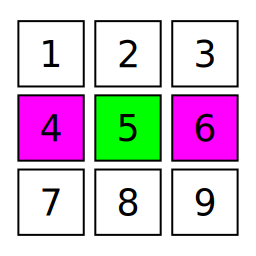
\includegraphics[width=0.8\textwidth]{assets/memory-access.pdf}
  \caption{Access pattern representation}
\end{figure}

The particular implementation for libdepixelize stores and access the elements
linearly like [1, 2, 3, 4, 5, 6, 7, 8, 9]. It could make good use of processor
cache, but ain't that easy. Suppose we are iterating on element 5, then we need
to access all its neighbours, but only neighbours 4 and 6 may be in cache,
especially in large images. This is the first problem in cache usage of the
implementation, but we cannot remove this usage pattern, because it's part of
the algorithm and there is a data dependency among the elements. However, we can
change the memory layout to favor the usage pattern. This technique is called
\href{http://en.wikipedia.org/wiki/Cache-oblivious_algorithm}{cache-oblivious
algorithm} and future versions of libdepixelize might implement it.

Another problem with the current data access pattern is that each element store
a complex object that may point to other regions of memory and add a level of
indirection that can contribute to cache miss. One idea that can increase the
cache hit is the one behind the
\href{http://stackoverflow.com/questions/10315041/meaning-of-acronym-sso-in-the-context-of-stdstring}{Small
String Optimization}. This change would highly increase data locality and fits
well in Kopf-Lischinski algorithm, because the complex objects stored by each
element in every phase tends to have a small maximum number of subelements.
